\documentclass[10pt,conference,compsocconf]{IEEEtran}

\usepackage{hyperref}
\usepackage{graphicx}
\usepackage[]{algorithm2e}
\usepackage{placeins}
\usepackage[english]{babel}
\usepackage[usenames, dvipsnames]{color}

\begin{document}
\title{Machine Learning - Project 1}
\author{
 Alexander Holloway - Bastian Nanchen - Arnaud Pannatier 
  \\
  \textit{Group : }Max and Lily learn ML \\
  \textit{EPFL 2017}
}
\maketitle

\begin{abstract}
Sentiment classification is an active area of research in the field of machine learning. Here, we present the results of a study into supervised learning methods for classifying the emotional senitment of Tweets -- either positive, or negative -- according to the presence of an emoticon. To this end, we leverage state-of-the-art pre-processing and feature engineering methods, and provide a comparison of learning methods that make use of the resultant features. Finally, we describe in detail the best model we identified for this purpose: \textcolor{blue}{Convolutional neural network, I suppose}, which achieved \textcolor{blue}{x accuracy} on unseen data.
\end{abstract}

\begin{description}
\item[Data] \ \\
Transforming the preprocessed text data into more practical format. 
\item[Preprocessing the data] \ \\
List of operation that was used to transform the raw data.
\item[Classification Methods] \ \\
Description of the different methods that were used as : Logistic regression, CNN, ...
\item[Results] \ \\
Presenation of the results of the differents methods.
\item[Discussion] \ \\
 A comment on the results and possible improvement.  
\end{description}

\section{Data}
\label{sec:data}

The data supplied through the online competition platform consists of 2.5 million labelled training examples, which take the form of Tweets that previously contained either positive or negative emoticons. The dataset is split down the middle, with 1.25 million training examples available for each class---positive and negative. Contrary to other similar classification tasks presented in the literature \cite{jiang2011target, tang2014learning}, there are no ``neutral'' class labels in this dataset. The absence of such indeterminate class labels allows us to formulate this problem as a binary classification task, which is advantageous.

Due to the nature of communication on the Twitter platform, the dataset contains many ``words'' that do not belong in a traditional English lexicon. Examples of these are usernames, URLs, hashtags, colloquialisms or slang, and typographical errors (both intentional and unintentional). Usernames and URLs were already stripped from the data, however the presence of other artefacts poses both issues and opportunities for this classification task. For example, the presence of repeated punctuation marks or characters may not make syntactic sense in traditional language, but more often than not, these artefacts have semantic meaning within a Tweet \cite{tang2014learning}. Similarly, hashtags can provide significant predictive power for the sentiment of phrase, without containing meaning in a pragmatic sense.

A detailed explanation of the specific language artefacts we processed, and the ways in which we leveraged them to improve classification performance is presented in Section \ref{sec:processing}.

\section{Feature processing}
\label{sec:processing}
In order to train learning models using the Twitter data, it was necessary to perform pre-processing to create useful features that characterise the two classes we seek to disambiguate. To this end, we employed pre-processing steps that broadly fit into three categories: Tweet transformation, transformation to word-embeddings, and transformation to ``Tweet-embeddings''.

\subsection{Tweet transformation}
The dataset that was provided had already undergone some basic pre-processing, but additional transformations were performed in order to improve our classification performance. The following transformations were inspired by the GloVe documentation \cite{glove}.

\subsubsection{Base transformations}
Each line of the provided data files represents one Tweet, with all words separated by a single whitespace. All URLs have been removed, and mentions of other users are replaced by the tag \texttt{<user>}. Necessarily, all emoticons have also been removed, however there is no indication of their presence within the original Tweet.

\subsubsection{Number transformation}
The idea is that all the numbers contained in a tweet have the same meaning for sentiment analysis. Therefore it makes sense to group them. To do that all the numbers are replaced with a tag: \texttt{<NUMBER>}

\subsubsection{Hashtag splitting}
Hashtags are a challenge to process in meaningful ways. A naive approach is to treat unique hashtags as different words in the vocabulary. Alternatively, if the hashtags can be split in an intelligent way, we can add signifcant meaning for the model.  Here, we replace the \# by the tag \texttt{<HASHTAG>} and then split all the remaining words on uppercase letters. In the event the hashtag is in all uppercase, the characters are not split, the words are left as is, and an additional tag \texttt{<ALLCAPS>} is added. For example the hashtag \texttt{\#ILikeMachineLearning} will be transformed to \texttt{<HASHTAG> I Like Machine Learning} and \texttt{\#ILIKEMACHINELEARNING} will be transformed to \texttt{<HASHTAG> ILIKEMACHINELEARNING <ALLCAPS>}. 

\subsubsection{Punctuation repetitions}
Some Tweets contain punctuation that is repeated at the end of a word. As before, it is more convenient to group similar expressions: \emph{i.e.} treat \texttt{!!!!!} the same way \texttt{!!!}, rather than treat them as two differents words. Therefore, each time a punctuation mark is repeated, it is transformed to \texttt{punctuation mark <REPEAT>}. 

\subsubsection{Elongated words}
In some tweets the last letter of some words is repeated. This is a similar problem than before. All these expressions should be treated as the same word in the vocabulary. In order to do so, all the repeated letters at the end of a word are replaced by a tag \texttt{<ELONG>}.

\subsubsection{Contractions and casing}
A final text processing step step is applied, where blank space is used to delimit contractions (\emph{i.e.} \texttt{'ll, 're, 'm, ...}) and and punctuation marks. In addition, all text is set to lowercase, in order to ensure that all phrases are evaluated equally regardless of casing during training.

\subsection{Word embeddings}
After the Tweets are modified in their original text format, it is necessary to transform them to a numerical format. Several methods exist for achieving this, \emph{e.g.} bag of words or $n$-gram representations. Recently, so-called ``word embedding'' formats \cite{} have been employed to great success in next classification tasks. In short, word embeddings map words to high-dimensional vectors that seek to characterise the words' usage in various semantic contexts. \cite{} Examples of their use in recent literature are manifold \cite{} and thus we investigated several variations of this representation.

Generally speaking, the advantage of using word embeddings, is that they allow all words in the vocabulary to be represented by vectors of uniform length. \emph{i.e.} given a vocabulary of $V$ words, and embeddings of dimensionality $D$, we create a $V \times D$ matrix of word embeddings that can be processed further.

\subsubsection{word2vec}
\texttt{word2vec} is a popular software tool used to create state-of-the-art word embeddings. \cite{mikolov2013distributed} It provides two embedding models: ``skip-gram'', and ``continuous bag of words'' (CBOW). The skip-gram model uses the current word of interest as input to a classifier that seeks to predict words within a certain range before or after it. The CBOW model does the opposite, by predicting the current word based on its textual context. The skip-gram architecture was found to perform better for semantic classification tasks, whereas CBOW performed better on syntactic classification. \cite{mikolov2013efficient} Given the task at hand, only skip-gram embeddings were evaluated in this task.

\subsubsection{GloVe}
GloVe (Global Vectors) is a word vector representation that was developed in the wake of \texttt{word2vec}'s popularity. GloVe creates word vectors via factorisation of a word co-occurrence matrix. At a high level, the GloVe algorithm works in three steps: computing co-occurence probabilities for all words $V$ in the vocabulary, and ratios of these probabilities with respect to other context words; applying some soft constraints upon word pairs in the form of linear biases; and computing the cost function with a weighting to prevent learning only from common word pairs. \cite{pennington2014glove}. The principal difference between GloVe and \texttt{word2vec} is that the first method use count-based occurence approach and the second used context-predictions to learn the vectors embeddings. 

\subsubsection{Sentiment-specific word embeddings}
The sentiment-specific word embedding (SSWE) method presented in \cite{tang2014learning} actually takes embeddings generated by other means as input, and modifies them in order to better capture the relative sentiment of words in the vocabulary. As an example, the SSWE representation seeks to represent the words ``good'' and ``bad'' as polar opposites---whereas methods such as GloVe or \texttt{word2vec} would map these words closely, as they are used in syntactically similar contexts. This transformation of embeddings is performed using a four layer neural network, and has been demonstrated as being more effective than standard word embeddings for the specific task of Tweet sentiment classification. \cite{tang2014learning}

\subsection{Tweet-embeddings}
Word-embedding representations create matrices of dimensionality $V \times D$ for $V$ words in a vocabulary, and $D$ elements per word vector. Tweets necessarily contain subsets of words in the vocabulary, and thus we must aggregate the embeddings for each subset of words, in order to construct an $N \times D$ feature matrix for $N$ tweets. To this end we trialled summation, and averaging of vectors to create a ``Tweet-embedding'' representation. In addition, weighted word-embeddings -- where the vector elements are inversely weighted according to frequency -- were evaluated, but the effects were negligible. \cite{schnabel2015evaluation} Finally, the mean of the word-embeddings for each Tweet was used.

\section{Classification methods}
Using the generated features 4 methods are applied to classify the data between happy tweets and sad ones. The three first are classic feature classifications that were applied to the tweets features. The last one is a more complex classification method and is directly applied on the embeddings.

\subsection{Logistic regression}
The first classifier that is applied is standard logistic regression. This classifier use the logistic function to determines whether the tweets belongs to one categories or another. This really simple method as the advantage that it is really fast to compute and easy to implement. It can be use to determine if the modification of the data processing as an impact on classification. But it will not be efficient enough to use for the competitions.

\subsection{SVM}
The more advanced classification technic of \textit{Support vector machine} is implemented as well. This method is often use in supervised learning. Given a set of training example belonging to two different categories, the SVM model build a frontier between the samples of the two categories with the biggest gap possible. This technics leads to better results for classification but also takes more times to run. 

\begin{figure}[h!]
\centering
	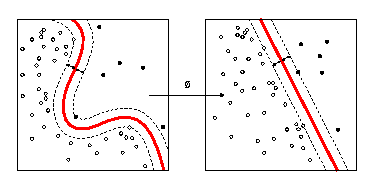
\includegraphics[scale=1.2]{SVM} 
\caption{The SVM model tries to find the frontier with the bigger gap possible.}
\label{plot:SVM}
\end{figure}
\FloatBarrier

\subsection{Regular neural networks}

Neural nets were also used on tweets features. This neural net has two layers of size TODO COMPLETE: (..,..). This was to take account that a neural network of  two layers is sufficient to represent any vectorial function.  If this technic was giving the best results of all the one that were used on on tweets representation, it didn't lead to the sufficiently good results for the competition. 

\subsection{Convolutional neural networks}

In order to achieve better classification, a convolutional neural network is applied. The idea is not just to look as the tweet as a vectorial sum of embeddings, but to consider their places in the tweets as well. In this case, all the tweets are represented by a matrix :  At each word of the tweet corresponds a line of the matrix, containing the embeddings of the words. This matrix has therefore a size of \texttt{(number of words in the tweet * dimension of embeddings)}. A first layer apply then the convolution, it creates some filters of given sizes (in our case 3,4,5), which will be slided over the tweets matrix. 


\begin{figure}[h!]
\centering
	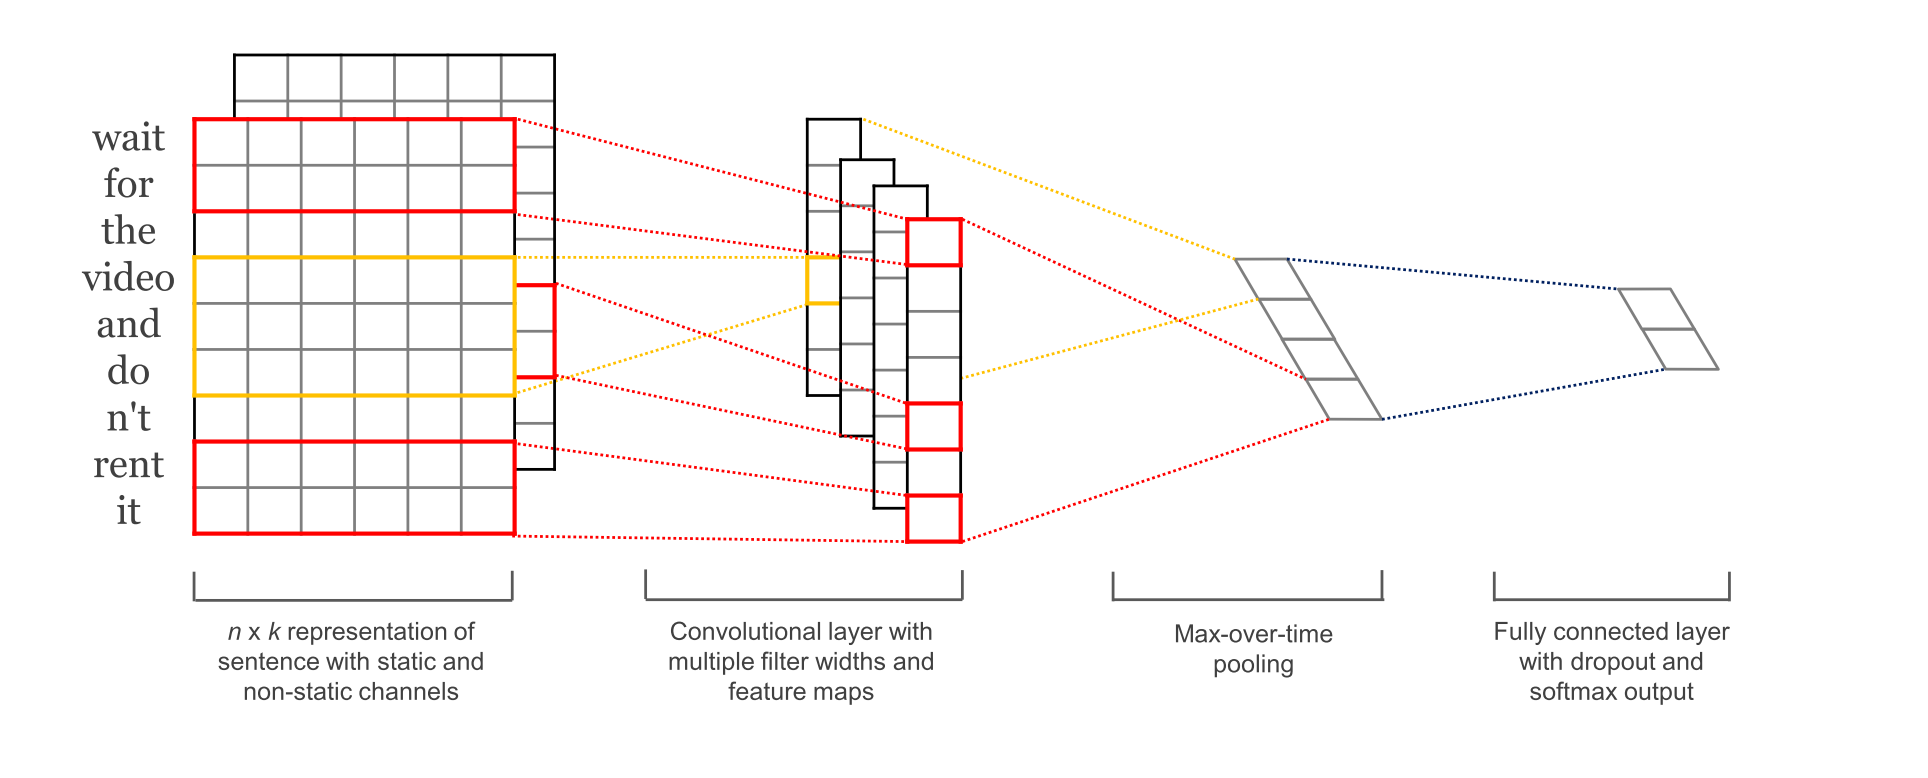
\includegraphics[scale=0.3]{CNN} 
\caption{Model of the convolutional neural network used for sentiment analysis}
\label{plot:CNN}
\end{figure}

\label{sec:methods}

\section{Results}
\label{sec:results}
\begin{figure}[h!]
\centering
	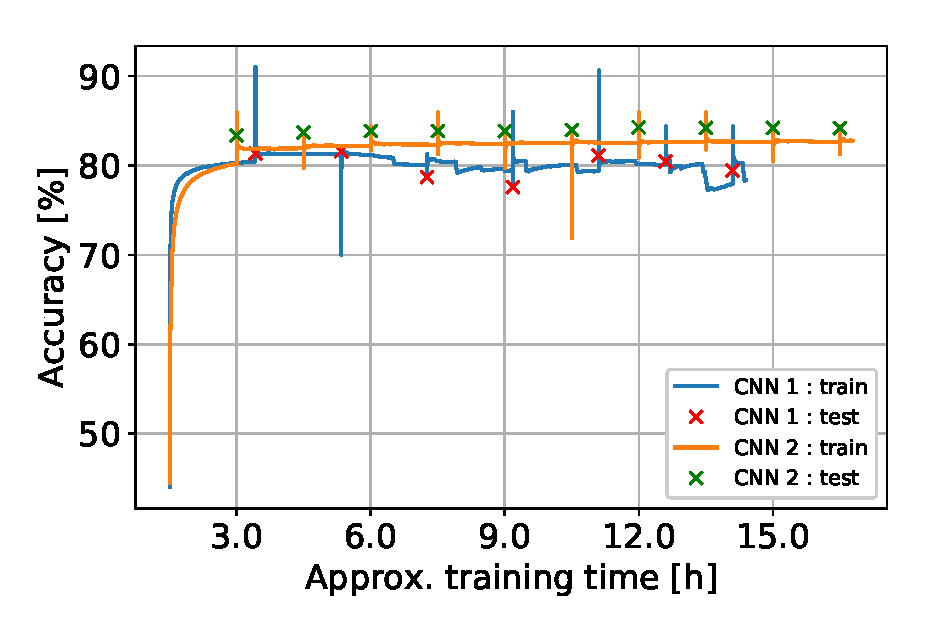
\includegraphics[scale=0.6]{CNNaccuracy} 
\caption{Training of the two convolutional neural nets. The first one does not use ``dropout'' as opposed as the second one.}
\label{plot:CNNaccuracy}
\end{figure}
\FloatBarrier


\begin{table}[h]
  \centering
  \begin{tabular}[c]{lllll}
    Input format&Model&Precision&Recall&Accuracy\\
    \hline
    Tweet-embed.&Logistic regression & 0.00       & 0.00  & 0.00 \\
    Tweet-embed.&SVM                 & 0.00       & 0.00  & 0.00 \\
    Tweet-embed.&Neural network	& 0.00	& 0.00	&	0.00 \\
    Word-embed.&CNN w.o. dropout                & 0.00	& 0.00	&	0.00 \\
    Word-embed.&CNN w. dropout & 0.00 & 0.00 & 0.00
    
  \end{tabular}
  \caption{Classification performances using local hold-out testing, for various input data formats.}
  \label{tab:results}
\end{table}



\section{Discussion}
\label{sec:discussion}

Here we have presented several methods of data pre-processing to create features from word-embeddings, and subsequently used these features to train a number of models. Empirically, we found that three different word-embeddings -- namely GloVe, skip-gram, and sentiment-specific -- gave comparable performance in the context of a Tweet sentiment classification task.

Classification performance was evaluated using four learning models: logistic regression, support vector machine, neural network, and convolutional neural network (CNN). Of these, all but the CNN took input in the form of word-embeddings which were aggregated per Tweet to create a so-called ``Tweet-embedding'' representation. The CNN accepted pre-trained word-embeddings that had not undergone such transformation, and in fact, achieved the best classification performance on an unseen test dataset.

There are many models for text classification outside of those explored here. Ultimately, classification performance on this task likely could be improved by using a pre-trained model (\emph{e.g.} Facebook's \texttt{fastText} \cite{joulin2016bag}), however, using a black box solution to maximise performance was not the aim of this project. When faced with similar tasks in the future, it would be illustrative to evaluate some of these ``out-of-the-box'' solutions, and explore their implementation details.


\bibliographystyle{IEEEtran}
\bibliography{report}

\end{document}
